\documentclass{article}
\usepackage[oldvoltagedirection]{circuitikz}
\usepackage[margin=1in]{geometry}
\usepackage{amsmath}
\usepackage{mathtools}
\usepackage{graphicx}
\setlength\parindent{0pt}

\title{Reti Logiche}
\author{}
\graphicspath{{img/}}

\begin{document}
\maketitle{}
23 Sep 2019, 16:14
\section{Propiet\'a delle reti loiche}

\begin{itemize}
    \item{Intrconnessione}
    \item{Scomposizione}
        Uno schema logico pu\'o essere rappresentato come composizione di reti pi\'u semplici, (si arresta quando si arriva a \textit{reti logiche elemnetari})
    \item{Elementari}
        Descrivono causa effetto
\end{itemize}

Nei sistemi pratici la storia passata del sistema deve essere rappresentata attraverso un insieme finito di segnali. (i.e. il numero passato di stati della rete deve essere finito) (slide 36. 01\_Modelli)

La funzione di uscita della rete dipende da ingresso corrente e stato interno della rete.

\begin{itemize}
    \item{Funzione di uscita o funzione macchina: $z(t) = f(x(t), y(t))$ (tabella, lookup-table)}
    \item{Next step function: $Y(t) = g(x(t), y(t))$, $g(x, y)$ chiamata \textbf{Funzione di stato}}
    \item{Funzione di marcatura dello stato: $y(t + \Delta t) = Y(t)$ o $y(t) = Y(t - \Delta t)$}
\end{itemize}

% Figura slide 40: Modello di mealy, funzioni caratteristiche, (quelle sopra)
\begin{circuitikz}
    \draw (0, 0) node[anchor=east]{x} -- (1, 0) to[twoport, t=$f$, >, number inputs=2] (2, 0) -- (3, 0) node[anchor=west]{z};
\end{circuitikz}

Nelle reti logiche combinatorie manca la dipendena dal tempo (slide 41)

Reti sequenziali corrispondono al modello generale, contengono retroazione e ritardi

% Figura slide 43: Blocco f corisponde ad una rete combinatoria
% Ingresso non cambia facendo cambiare l'uscita, cambia facendo variare le variabili di stato. Una rete di questo modo viene chiamata "Modello di Moore"
% Una rete di questo tipo e' ancora una rete sequenziale

%es:
Rete senza ingressi provenienti dall'eseterno viene chiamata: rete autonoma.  ($y(t) = y(t+1)$: la rete \'e costante).
Altra alternativa \'e un comportamento ciclico.

%%% Guarda se togliere
Se:
$z = f(x)$ e $Y= g(x, y)$: rete combinatoria, dipende solo da $z$


Rete sequenziale con ingresso non attaccato a $g$ \'e rete combinatoria (sostituire con figura)

Rete sequenziale con uscita non attaccata a $g$ \'e rete combinatoria (sostituire con figura)

Sintesi multiuscita pg. 29 slide \_2\_RetiCombinatorie\_I\_parte

Numero funzioni di $n$ variabili $F(n) = 2^{2^n}$, slide 30

\begin{center}
    \begin{tabular}{c c c|c}
        $x_1$ & $x_2$ & $x_3$ & $f$\\
        \hline{}
        0 & 0 & 0 & 0\\
        0 & 0 & 1 & 0\\
        0 & 1 & 0 & 0\\
        0 & 1 & 1 & 1\\
        \hline{}
        1 & 0 & 0 & 0\\
        1 & 0 & 1 & 1\\
        1 & 1 & 0 & 1\\
        1 & 1 & 1 & 1\\
    \end{tabular}
\end{center}

Metodo somma di prodotti: prendo solo righe con 1, le scrivo come prodotti e le sommo

\[
    \begin{rcases}
        f_3 = \bar{x_1} x_2 x_3\\
        f_5 = x_1 \bar{x_2} x_3\\
        f_6 = x_1 x_2 \bar{x_3}\\
        f_7 = x_1 x_2 x_3
    \end{rcases}
    f =  \bar{x_1} x_2 x_3 + x_1 \bar{x_2} x_3 +  x_1 x_2 \bar{x_3} + x_1 x_2 x_3
\]

Applicbile a qualsiasi tabella combinatoria ( Espressione canonica \textit{sum of products} SP)


\subsection{Espressione canonica Prodotto di Somme: PS}

Data una tabella della verit\'a, consideriamo gli zeri della funzione (OFF-set). Per ogni zero possiamo costruire un termine somma in cui compaiono come variabili dipendenti tutte le variabili della funzione di partenza.
Le variabili compaiono in forma vera se compaiono come zeri, vengono prese in forma complementata se compaiono come 1 nella riga della tabella.

\[
    \begin{rcases}
        s_0 = x_1 x_2 x_3\\
        s_1 = x_1 x_2 \bar{x_3}\\
        s_2 = x_1 \bar{x_2} x_3\\
        s_4 = \bar{x_1} x_2 x_3
    \end{rcases}
    S =  (x_1 x_2 x_3)(x_1 x_2 \bar{x_3})(x_1 \bar{x_2} x_3)(\bar{x_1} x_2 x_3)
\]

% Equivalenza espressioni booleane - Reti Combinatorie (Slide 50)
% Manca Conta porte logiche N_op = 5 e N_M = 16
Si riescono a sintetizzare reti pi\'u ottimizzate attraverso le mappe di Karnugh o alg. Quiaf-McCluskeyt

N letterari: si applica su soltanto al max 2 livelli. Conta il numero di morsetti del $1^o$ livello (somma: $N_{let}$ = 12, prodotto 12, altro 6)

\section{24 Sep 2019,  9:02}
% Definizione min e max termine slide: reti combinatorie parte 2
Prendendo in considerazione l'esempio del Full-Adder (slide 4)
\subsection{Espressione canonica \textit{SoP} delle funzioni $S_0$ e $C_1$}
$S_0 = \bar{x_0} \bar{y_0} c_1 + \bar{x_0} y_0 \bar{c_0} + x_0 \bar{y_0} \bar{c_0} + x_0 y_0 c_0 = m_1 + m_2 + m_4 + m_7 = \sum m_3(1, 2, 4, 7)$\\
$C_1 = \bar{x_0} y_0 c_0 + x_0 \bar{y_0} c_0 + x_0 y_0 \bar{c_0} + x_0 y_0 c_0 = m_3 + m_5 + m_6 + m_7 = \sum m_3(3, 5, 6, 7)$

Un modo pi\'u preciso sarebbe: $S(x_0, y_0, c_0) $, esplicitando l'ordine in cui vengono prese le variabili

$\sum m_3$ indica la sommatoria dei mintermini di 3 variabili


\subsection{Espressione canonica \textit{PoS}}

$S_0 (x_0, y_0, c_0) = (x_0 + y_0 + c_0) (x_0 + \bar{y_0} + \bar{c_0}) (\bar{x_0} + y_0 + \bar{c_0}) (\bar{x_0} + \bar{y_0} + c_0) = M_0 M_3 M_5 M_6 = \prod M_3(0, 3, 5, 6)$


\subsection{Teorema di Shannon}
Ogni espressione logica di $n$ variabili pu\'o essere espressa come:

\[f(x_1, x_2, \ldots, x_n) = x_1 \cdot f(0, x_2, \ldots, x_n) + x_1 \cdot f(1, x_2, \ldots, x_n)\]

Dall'espressione di una funzione riusciamo a riottenere la somma dei mintermini, utilizzando il th.\ di Shannon:

\[
    \begin{split}
        z &= x_1 x_2 + x_1 x_3 + x_2 x_3 = \\
         &= \bar{x_1} ( 0 \cdot x_2 + 0 x_3 + x_2 x_3) + x_1 (1 x_2 + 1 x_3 + x_2 x_3) = \\
         &= \bar{x_1} (x_2 x_3) + x_1 (x_2 + x_3 + x_2 x_3) = \\
         &= \bar{x_2} (x_1 (0 x_3) + x_1 (0 + x_3 + 0 x_3)) + x_2 (\bar{x_1} (1 x_3) + x_1 (1 + x_2 + 1 x_3)) =\\
         &= \bar{x_2} (x_1 x_3) + x_2 (\bar{x_1} x_3 + x_1) =\\
         &= \bar{x_3} (\bar{x_2} x_1 0 + x_2 \bar{x_1} 0 + x_2 x_1) + x_3 (\bar{x_2} x_1 1 + x_2 \bar{x_1} 1 + x_2 x_1) =\\
         &= \bar{x_2} x_2 x_1 + x_3 \bar{x_2} x_1 + x_3 x_2 \bar{x_1} + x_3 x_2 x_1 =\\
         &= m_3 + m_5 + m_6 + m_7
  \end{split}
  \]


Le leggi di de morgan dimostrano che le famiglie (And-Not) e (Or-Not) sono funzionalmente complete.

% TODO: Immagine circuito
% TODO: Immagine decoder con mintermini

DECODER: ad $n$ ingresi corrispondono $2^n$ uscite

\begin{figure}[h]
    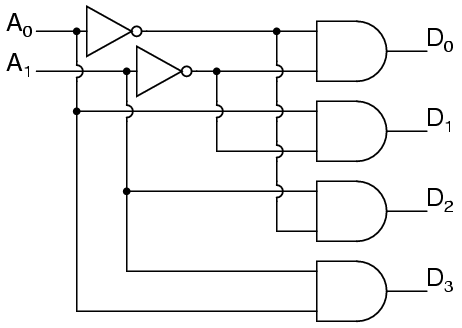
\includegraphics[width=0.4\textwidth]{decoder}
    \centering
    \caption{decoder}
\end{figure}
% TODO: Immagine decoder con MAXTERMINI (Decoder 3:8 a OR)
% TODO: De morgan con OR (ingresso al centro negato) -> AND negati invertiti
% Simbolo nand si puo fare con frecce
% TODO: Decoder a nand (produce MAXTERMINI)

\textbf{Espressione generale SP}: $f(x_{n-1}, \ldots, x_1, x_0) = \sum_{i=0, 2^n -1} m(i) f(i)$

\textbf{Espressione generale PS}: $f(x_{n-1}, \ldots, x_1, x_0) = \prod_{i=0, 2^n -1} (M(i) +f(i))$

%TODO: foto multiplexer a 8 canali con 3 var di selezione del canale Aggiungendo valori della funzione con carry out guarda foto
Il decoder sta in corrispondenza con le espressioni canoniche, il multiplexer sta un corrispondenza con le espressioni generali.
\end{document}
